\section{Benchmarking}
There are several key parts of the website that we found would benefit from benchmarking. These sections include the landing page, product page and the search results. 

These pages are very important for the user experience but are also well defined in the online commerce space. 
\subsection{Landing page}
For the landing page, we take a look at Craigslist and Bland.is.
These websites are those we will draw large inspirations from and it is important to view their differences closely. \textit{See figures 1 and 2}

\begin{Figure}
    \begin{center}
        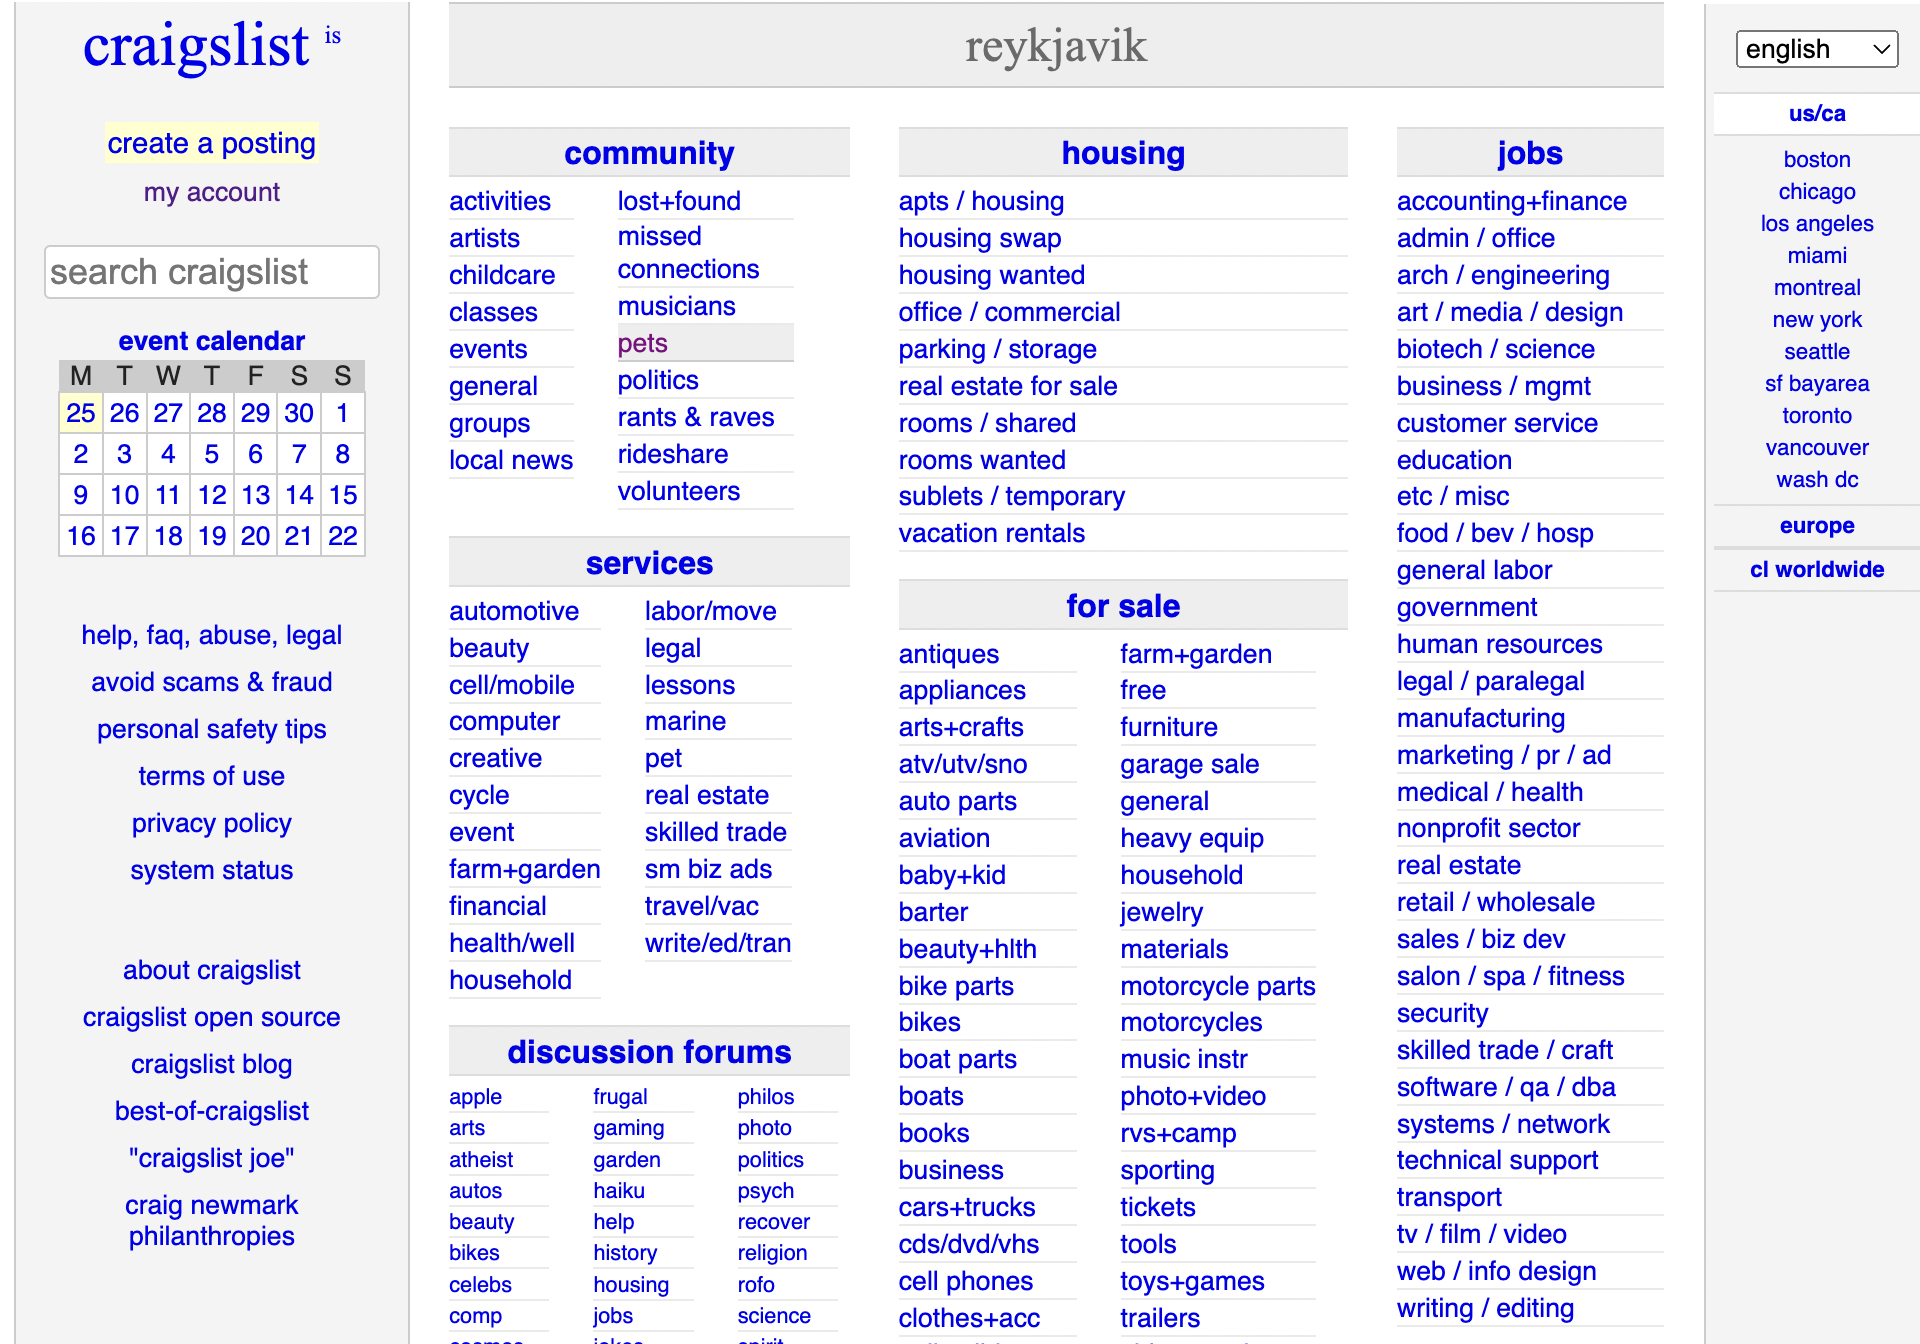
\includegraphics[width=150mm, height=80mm]{Images/benchmarking/landing_page_cl.png}
\captionof{figure}{Craigslist Landing page}
    \end{center}
\end{Figure}
\begin{Figure}
    \begin{center}
        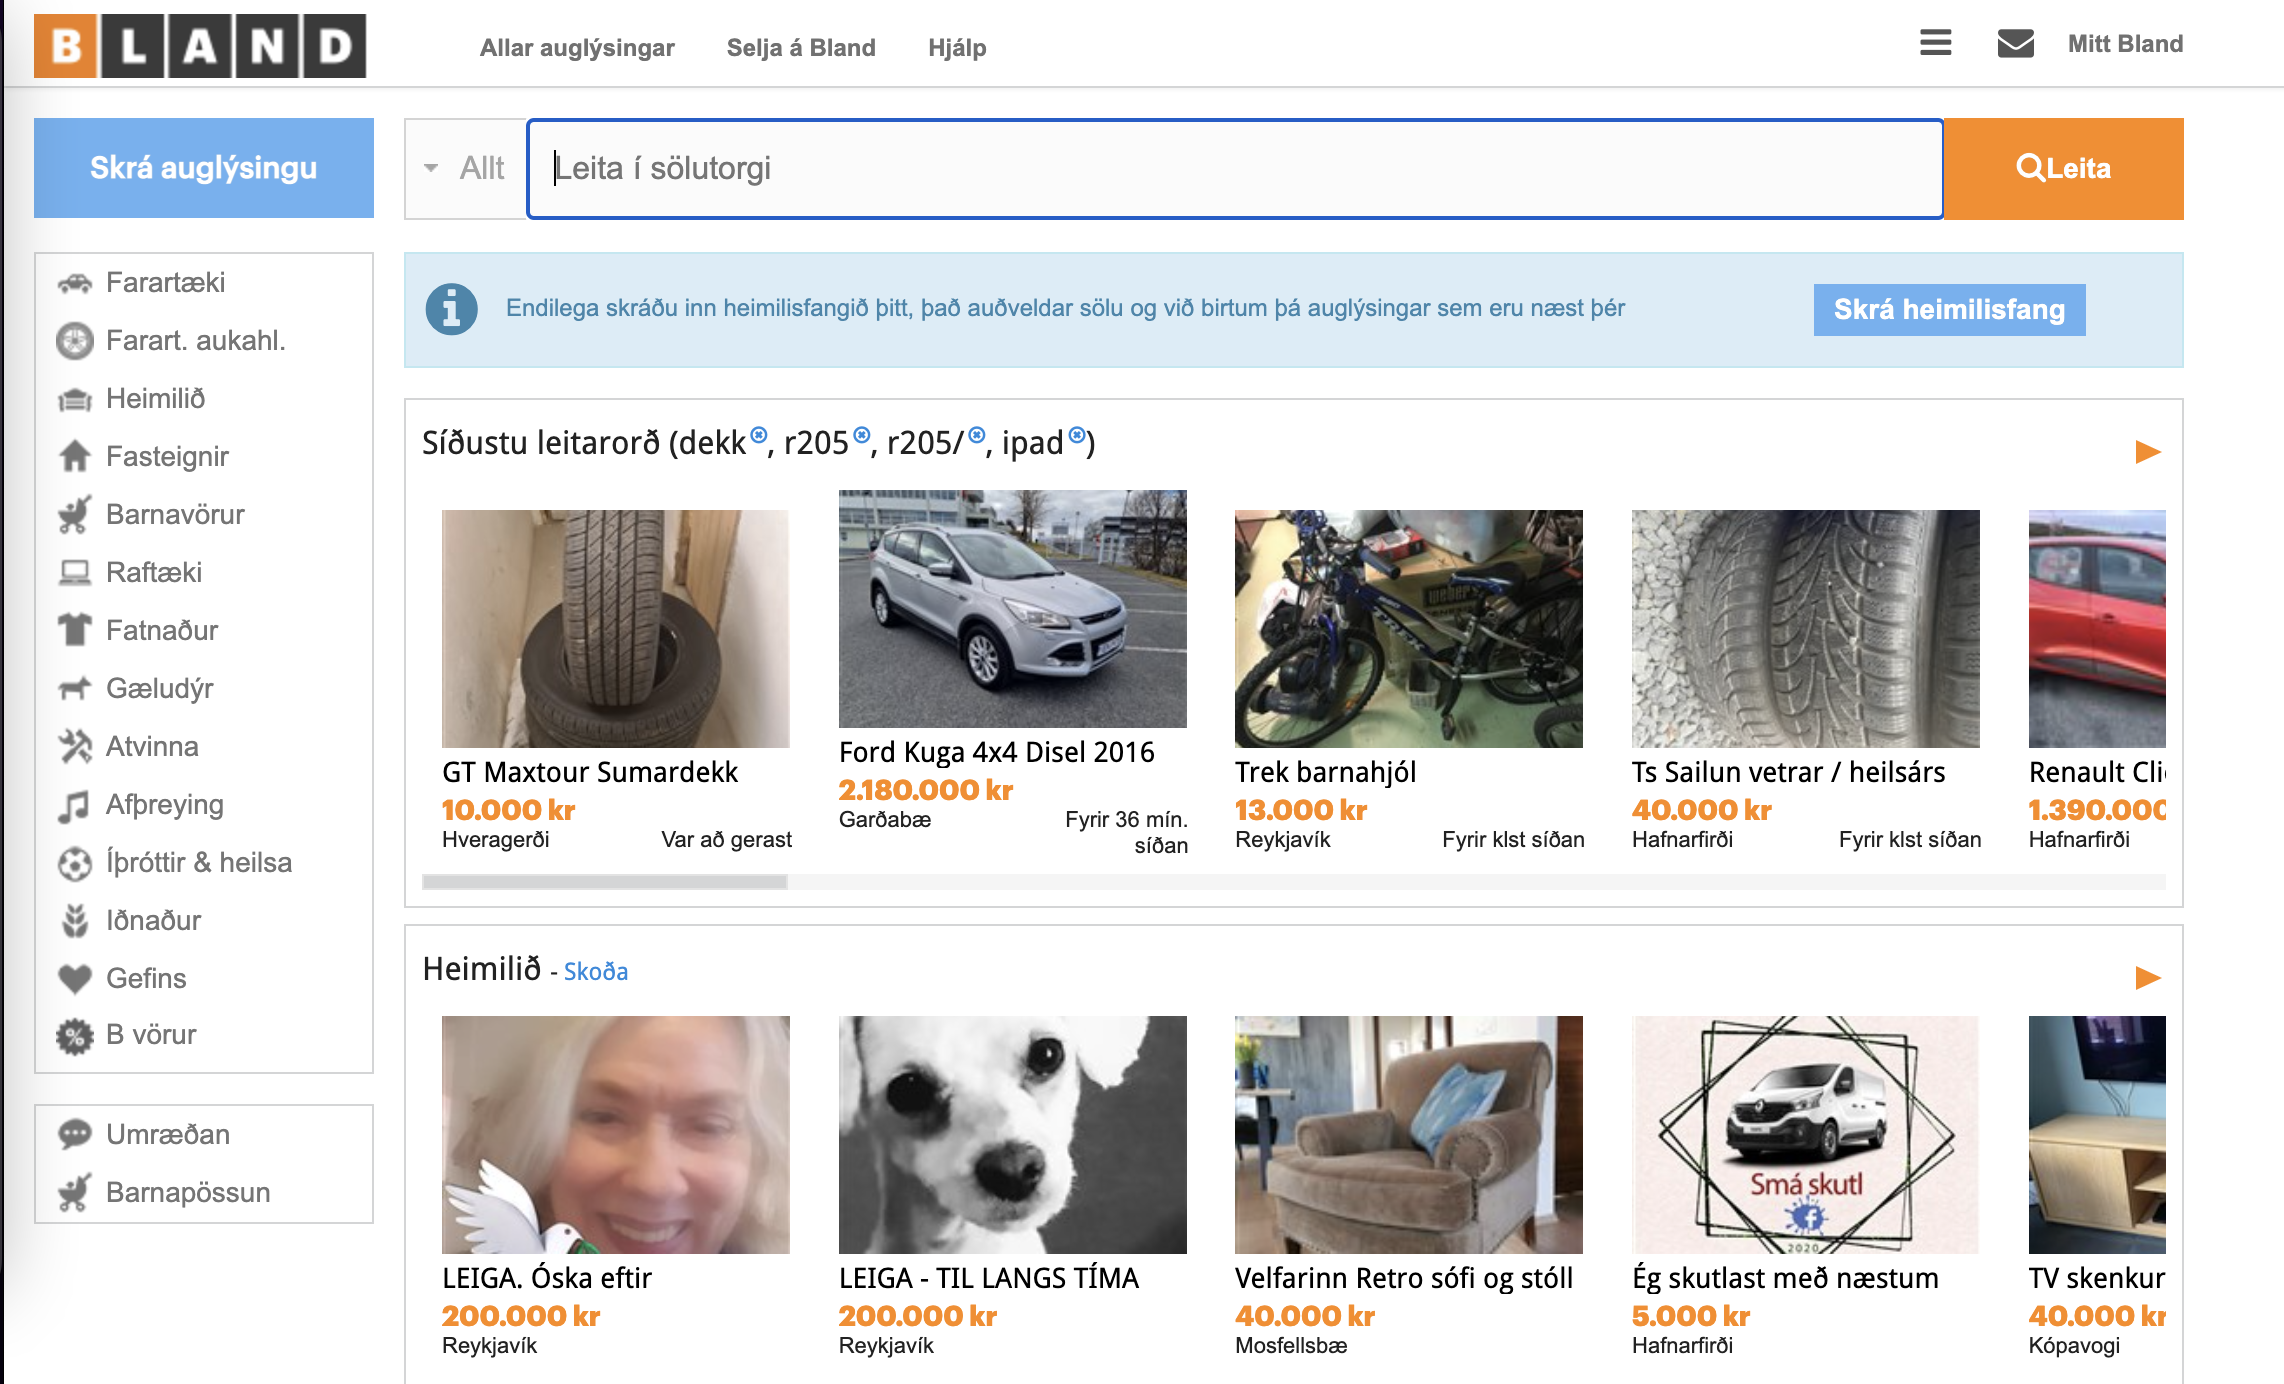
\includegraphics[width=150mm, height=80mm]{Images/benchmarking/landing_page_bland.png}
\captionof{figure}{bland.is Landing page}
    \end{center}
\end{Figure}

Right of the bat, we notice that Craigslist focuses on access to categories and sub-categories whilst bland puts their focus on showing you relevant products you might want to view, utilizing the users recent searches to achieve that.
The search bar is prominent for Bland but for Craigslist, it sort of hides in the UI, rather placing the users' focus on navigating through the categories first. 

\subsection{Product page}
The product page is the last step for the user before checkout. Therefor, important that if the product page sells the user on the product, the checkout process can begin, which is our goal. 

For the product page to be able to sell the user on the product, the most relevant information needs to be clearly visible on their first look. We continue to use Bland and Craigslist for our benchmark, with the edition of a product page from Elko's website. \textit{See figures 3, 4, 5}
\begin{Figure}
    \begin{center}
        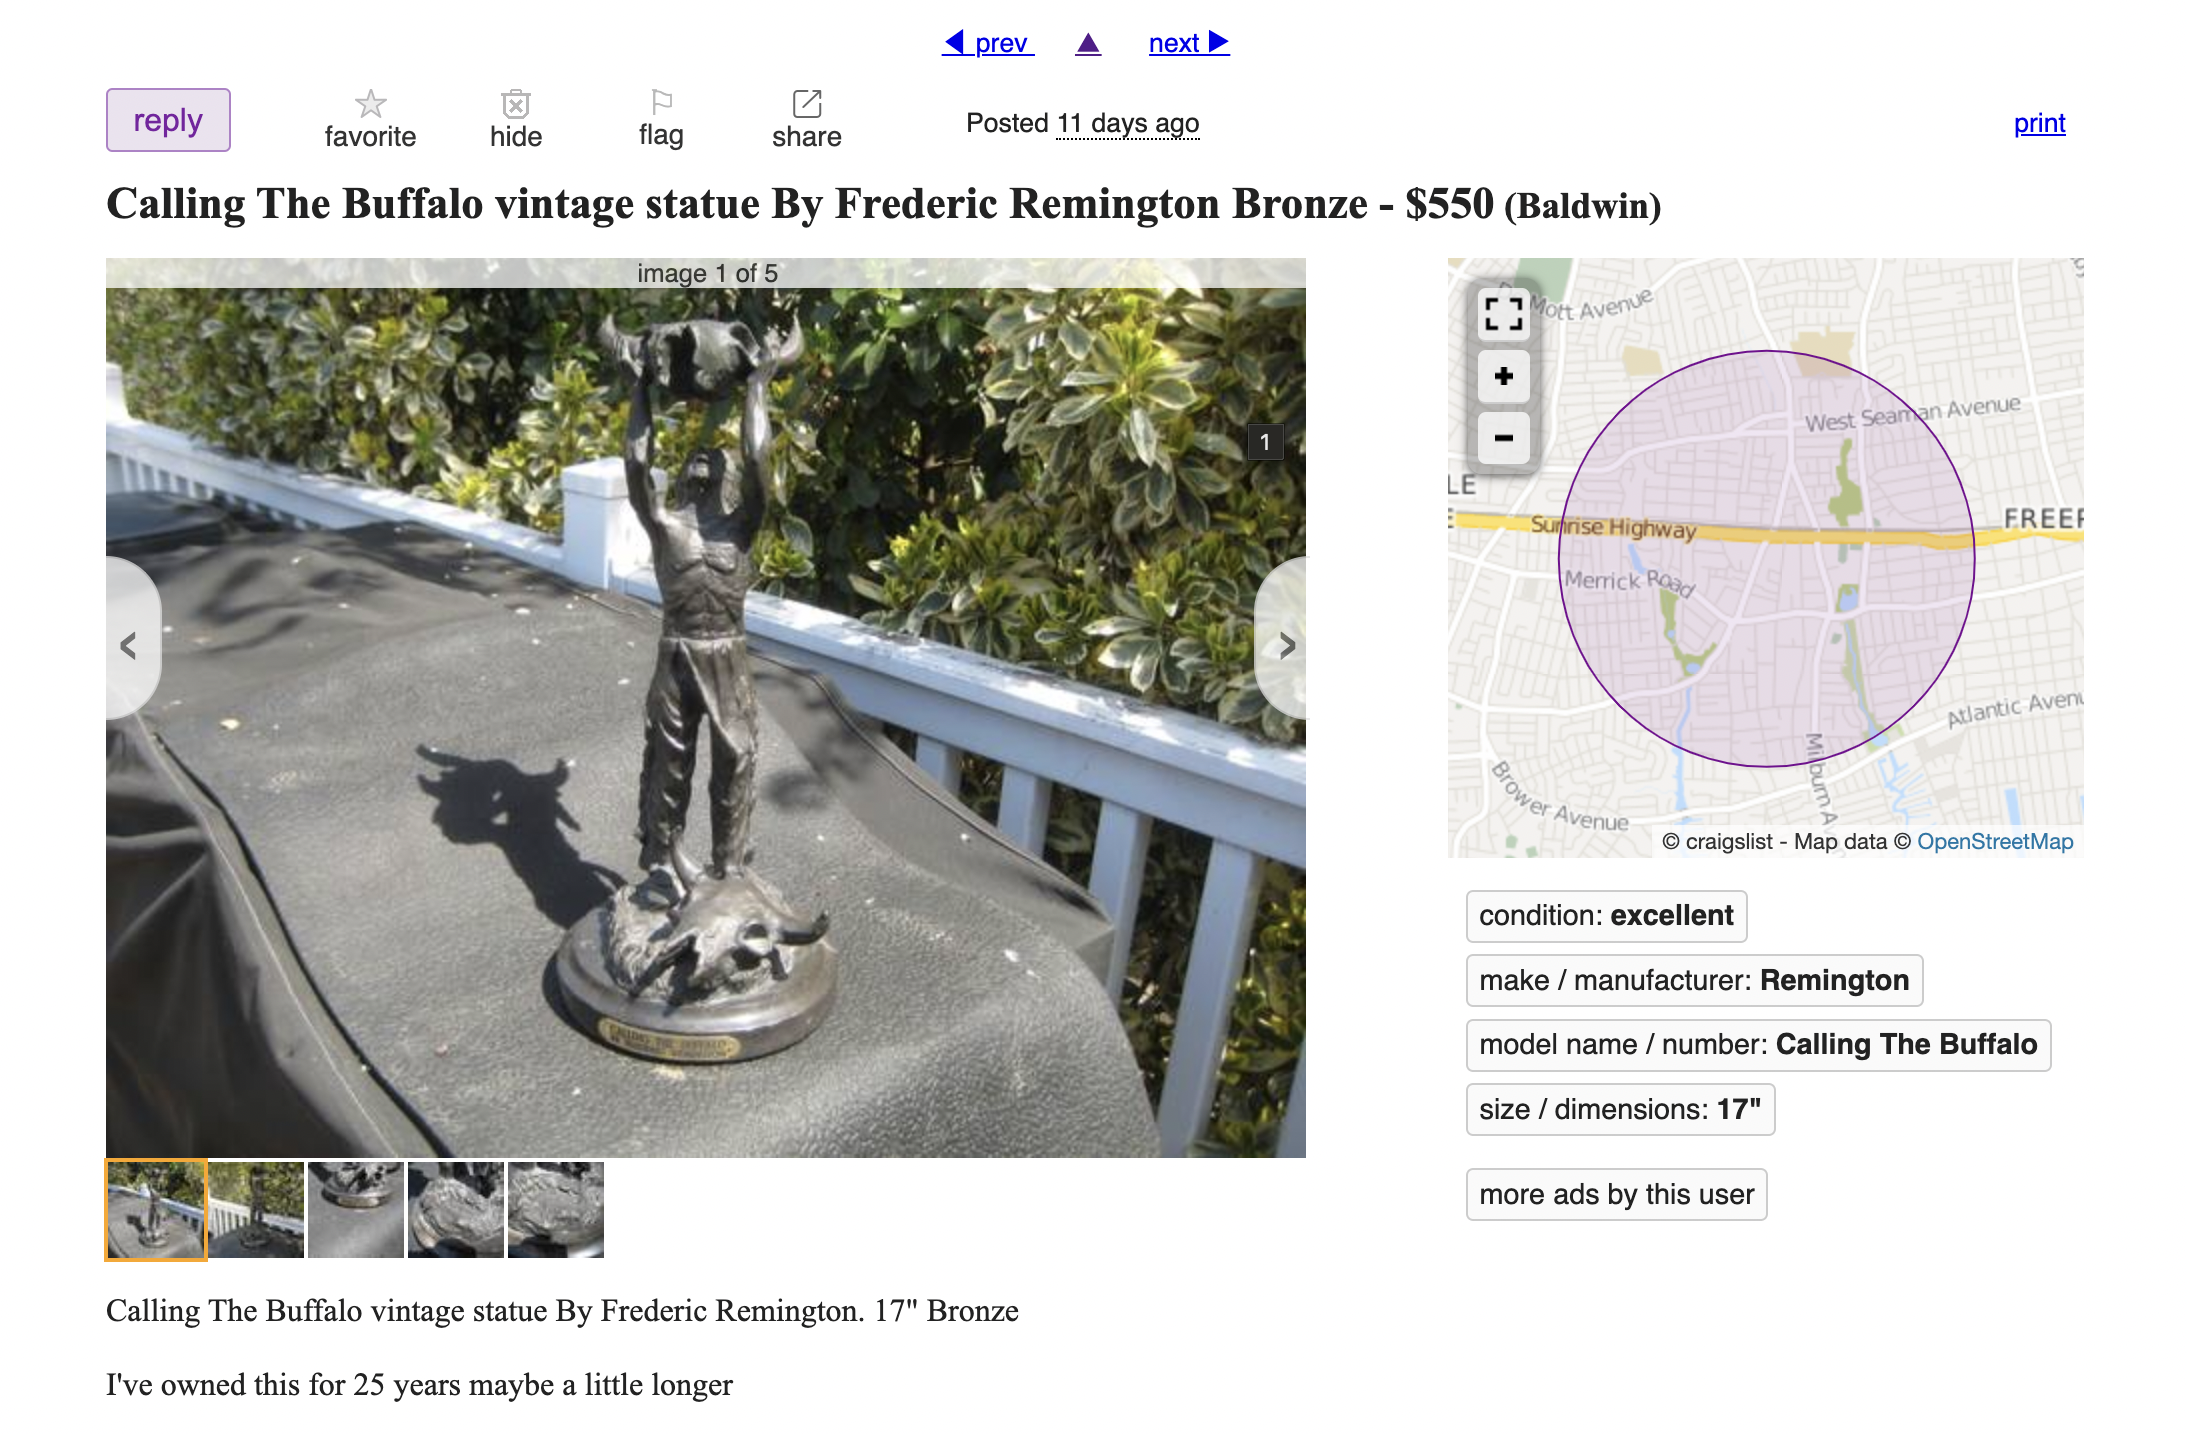
\includegraphics[width=150mm, height=80mm]{Images/benchmarking/product_page_cl.png}
\captionof{figure}{Craigslist Product page}
    \end{center}
\end{Figure}
\begin{Figure}
    \begin{center}
        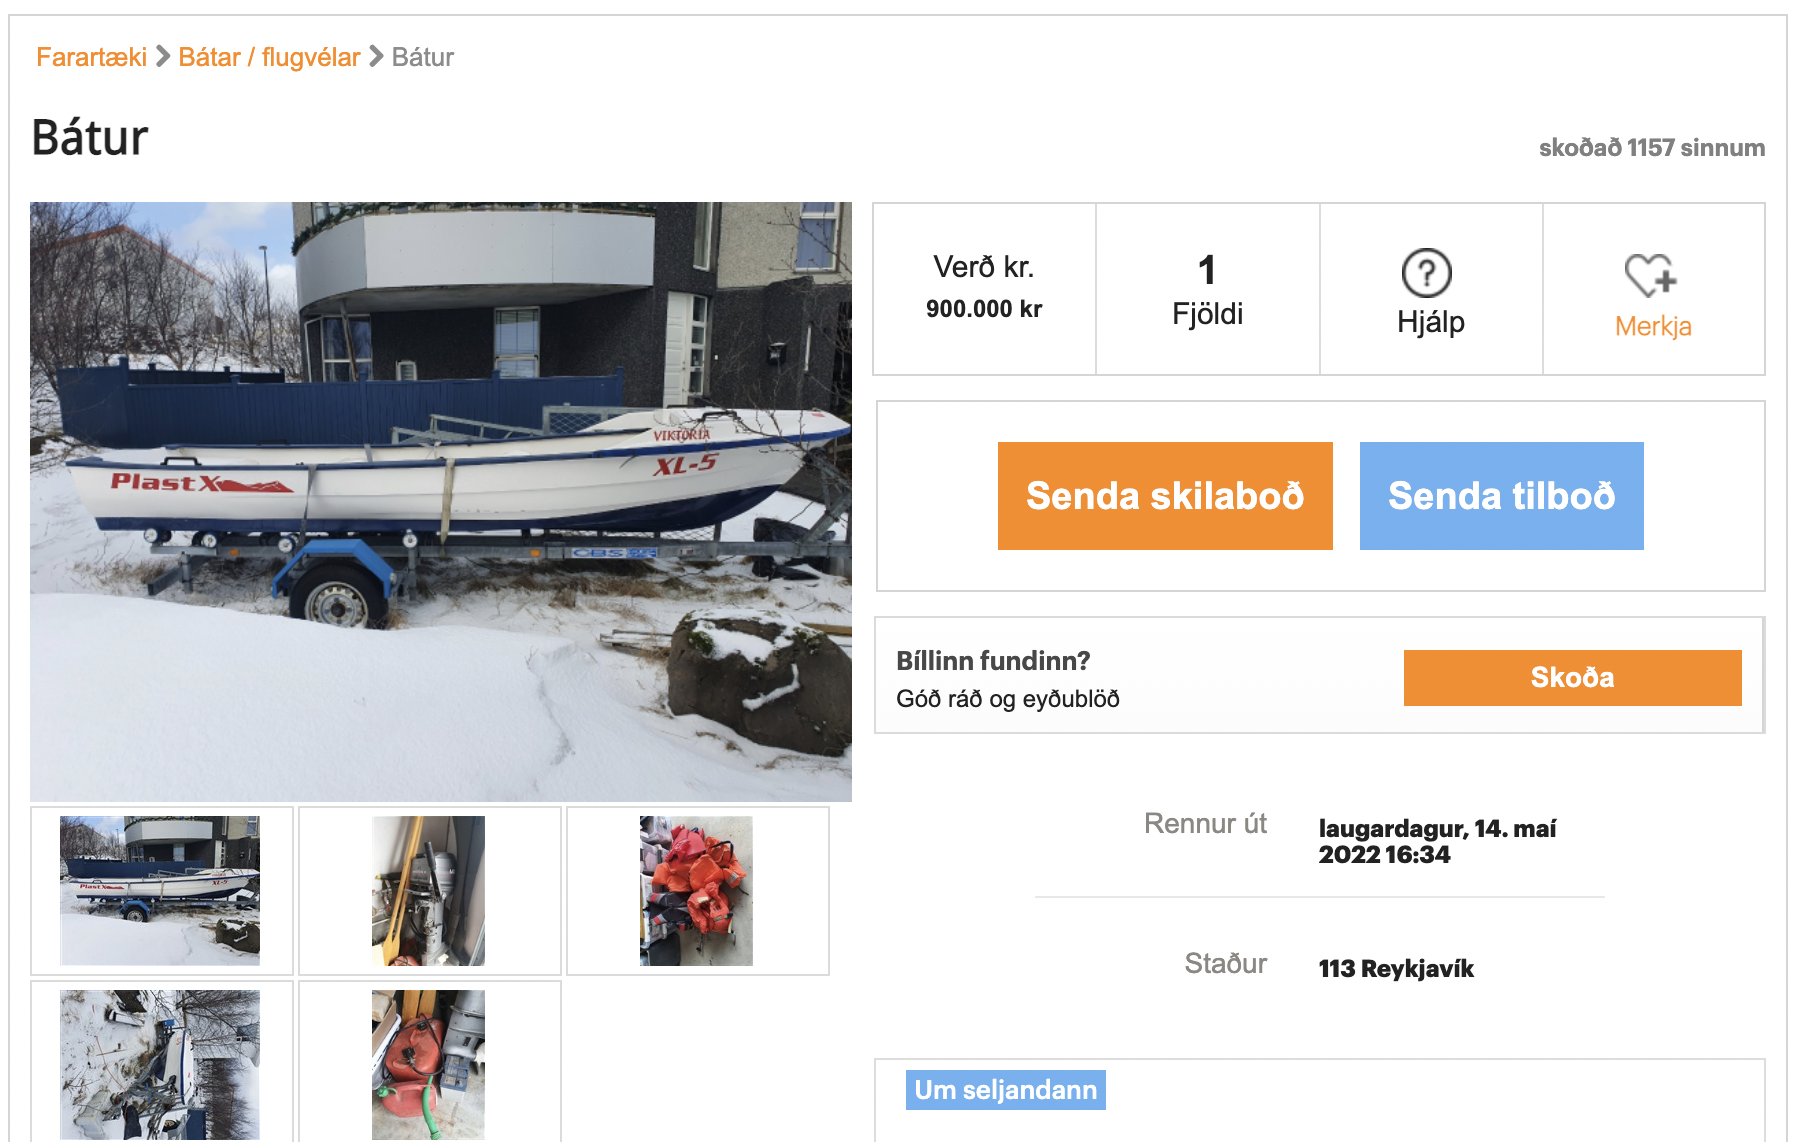
\includegraphics[width=150mm, height=80mm]{Images/benchmarking/product_page_bland.png}
\captionof{figure}{bland.is Product page}
    \end{center}
\end{Figure}
\begin{Figure}
    \begin{center}
        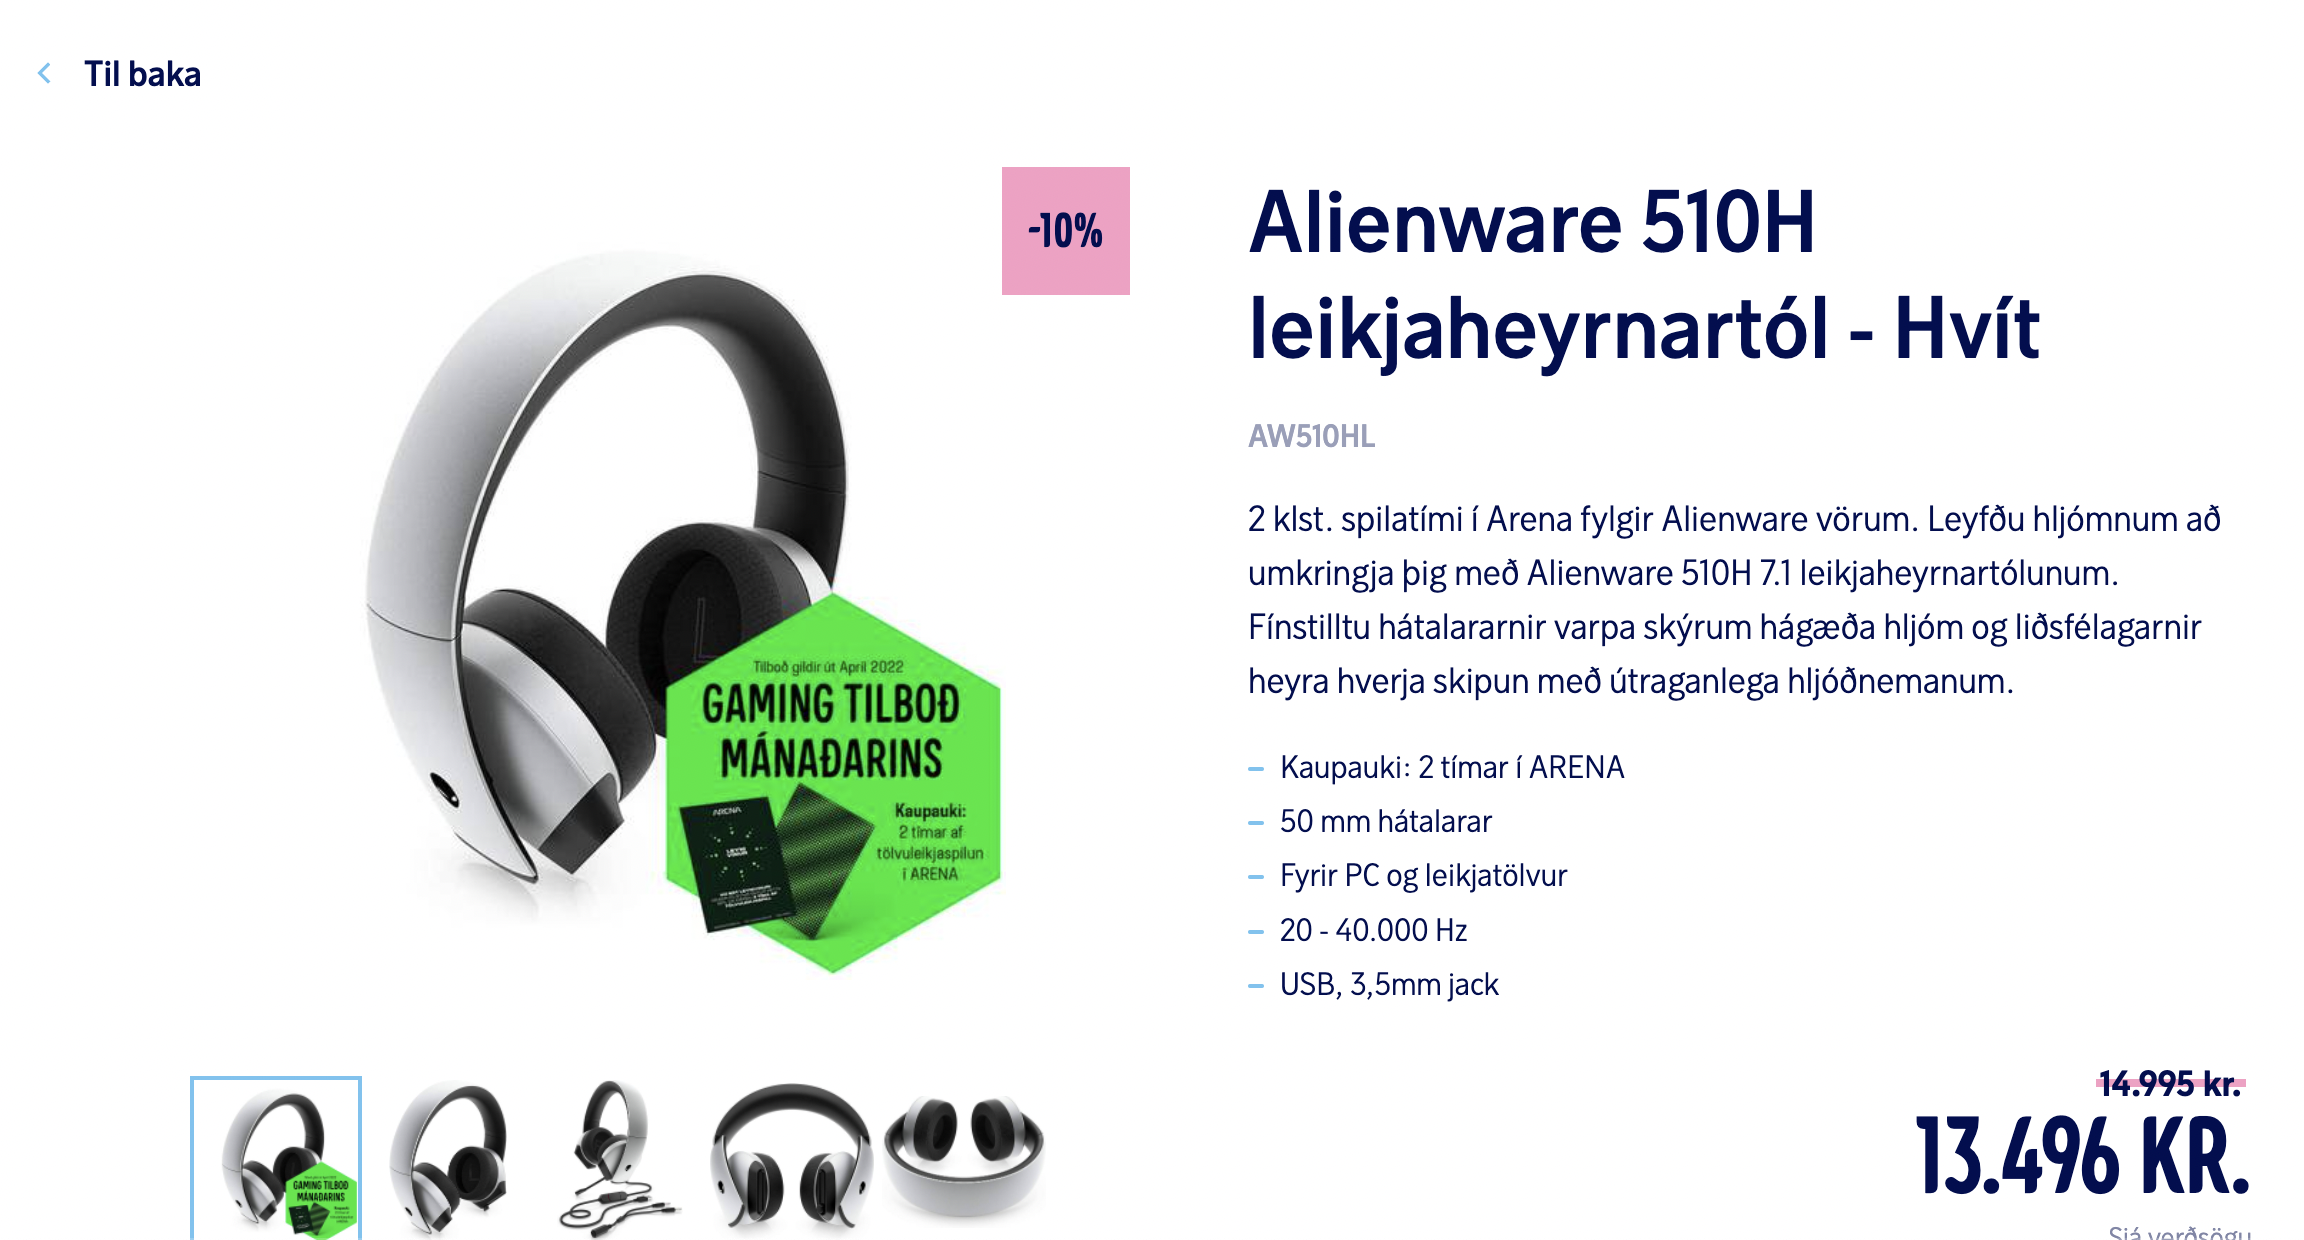
\includegraphics[width=150mm, height=80mm]{Images/benchmarking/product_page_elko.png}
\captionof{figure}{bland.is Product page}
    \end{center}
\end{Figure}
Omitted in the product page screenshot is the side and navigation bar, as we want to focus on the information on the product page.
Something that all these product pages have in common is the image gallery, Big emphasis is on the product images, and all but Elko put focus away from the item description. Craigslist, focusing on location and Bland focusing on doing an action. Elko has a small sale pitch with some key notes.

Viewing these screenshots in a small window, Elko has some nice features, that really show how they emphasise on the name of the product, an image and the price. All of these features, sans the image, are harder to make out in the other examples.

\subsection{Search results}
Search results give us what we want, hopefully. The play a key role in any data driven website and must be thought about carefully. 

As always, we base our benchmark on Craigslist and Bland, with the addition of Ebay. \textit{see figures 6, 7, 8}

\begin{Figure}
    \begin{center}
        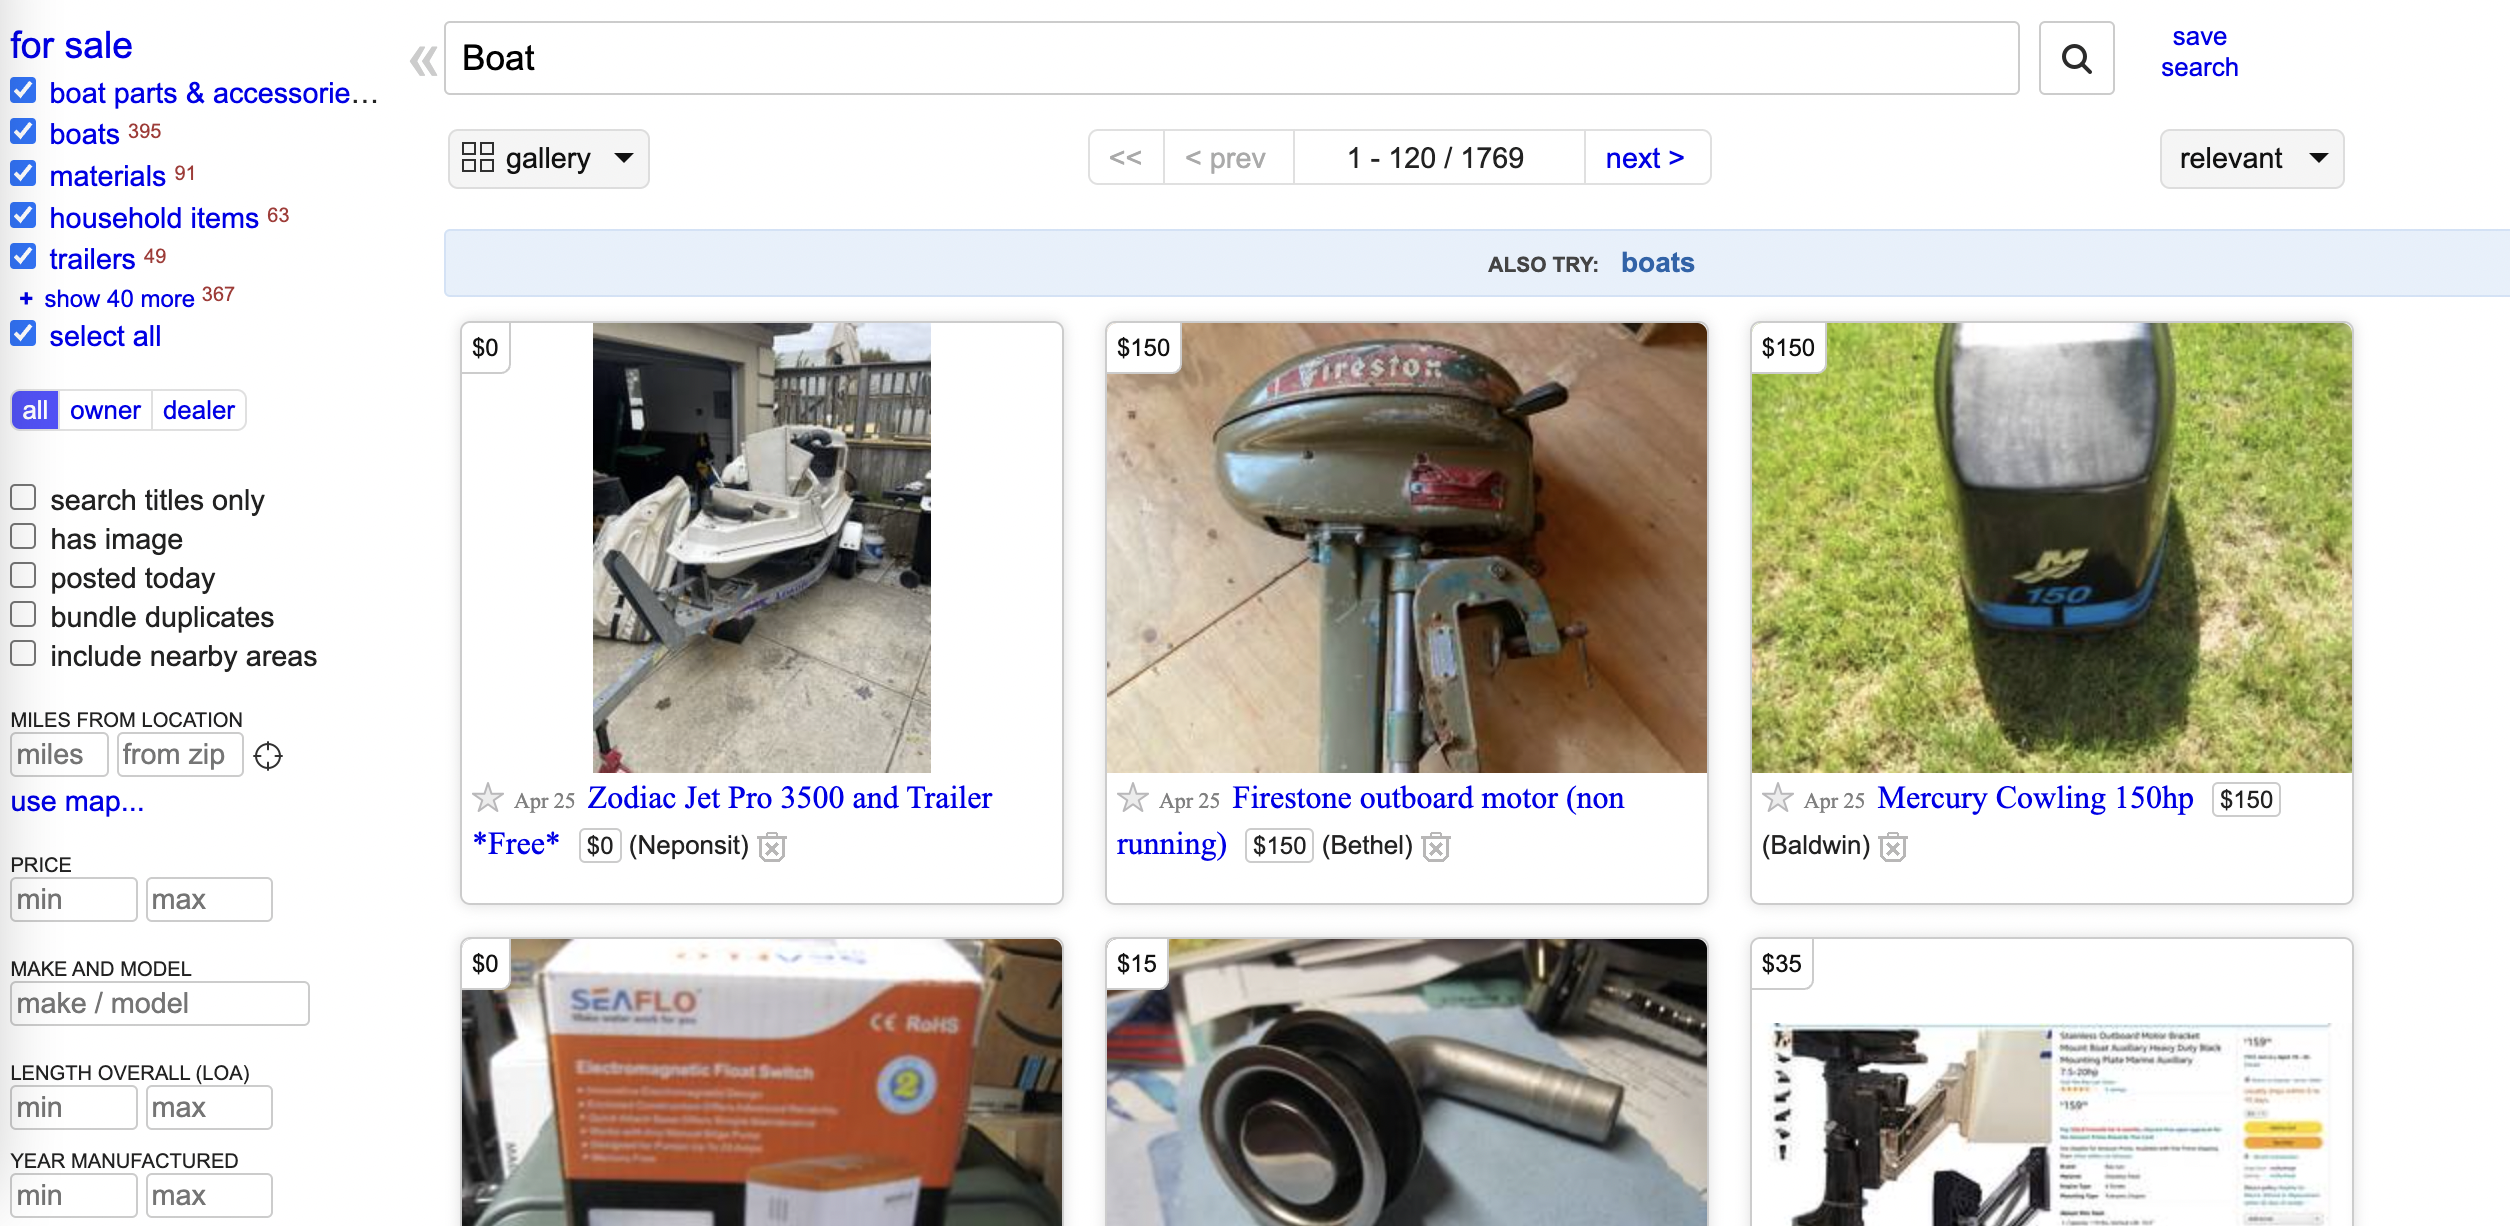
\includegraphics[width=150mm, height=80mm]{Images/benchmarking/search_result_cl.png}
\captionof{figure}{Craigslist search result page}
    \end{center}
\end{Figure}
\begin{Figure}
    \begin{center}
        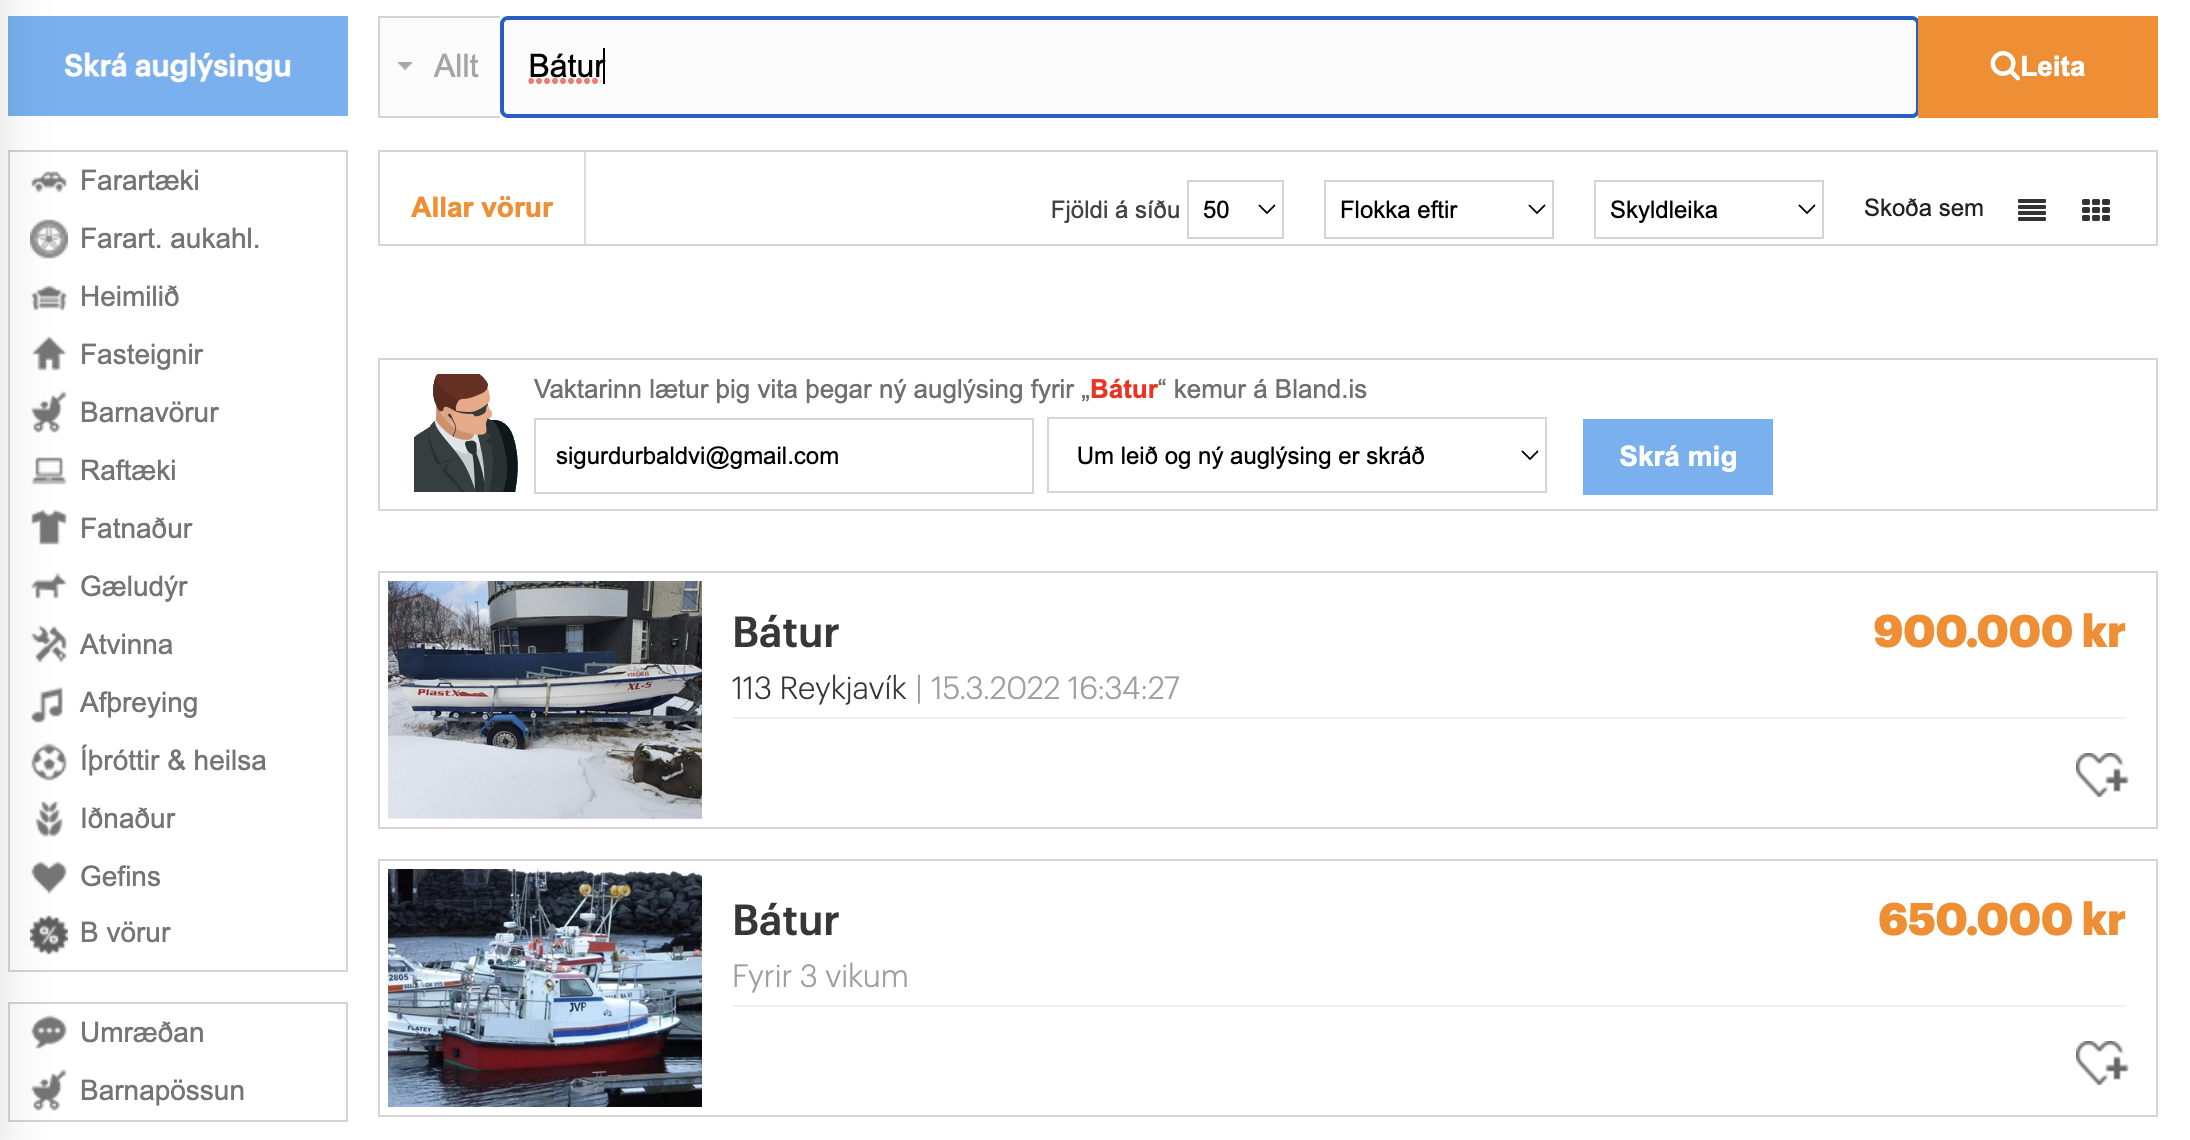
\includegraphics[width=150mm, height=80mm]{Images/benchmarking/search_result_bland.png}
\captionof{figure}{Bland.is search result page}
    \end{center}
\end{Figure}
\begin{Figure}
    \begin{center}
        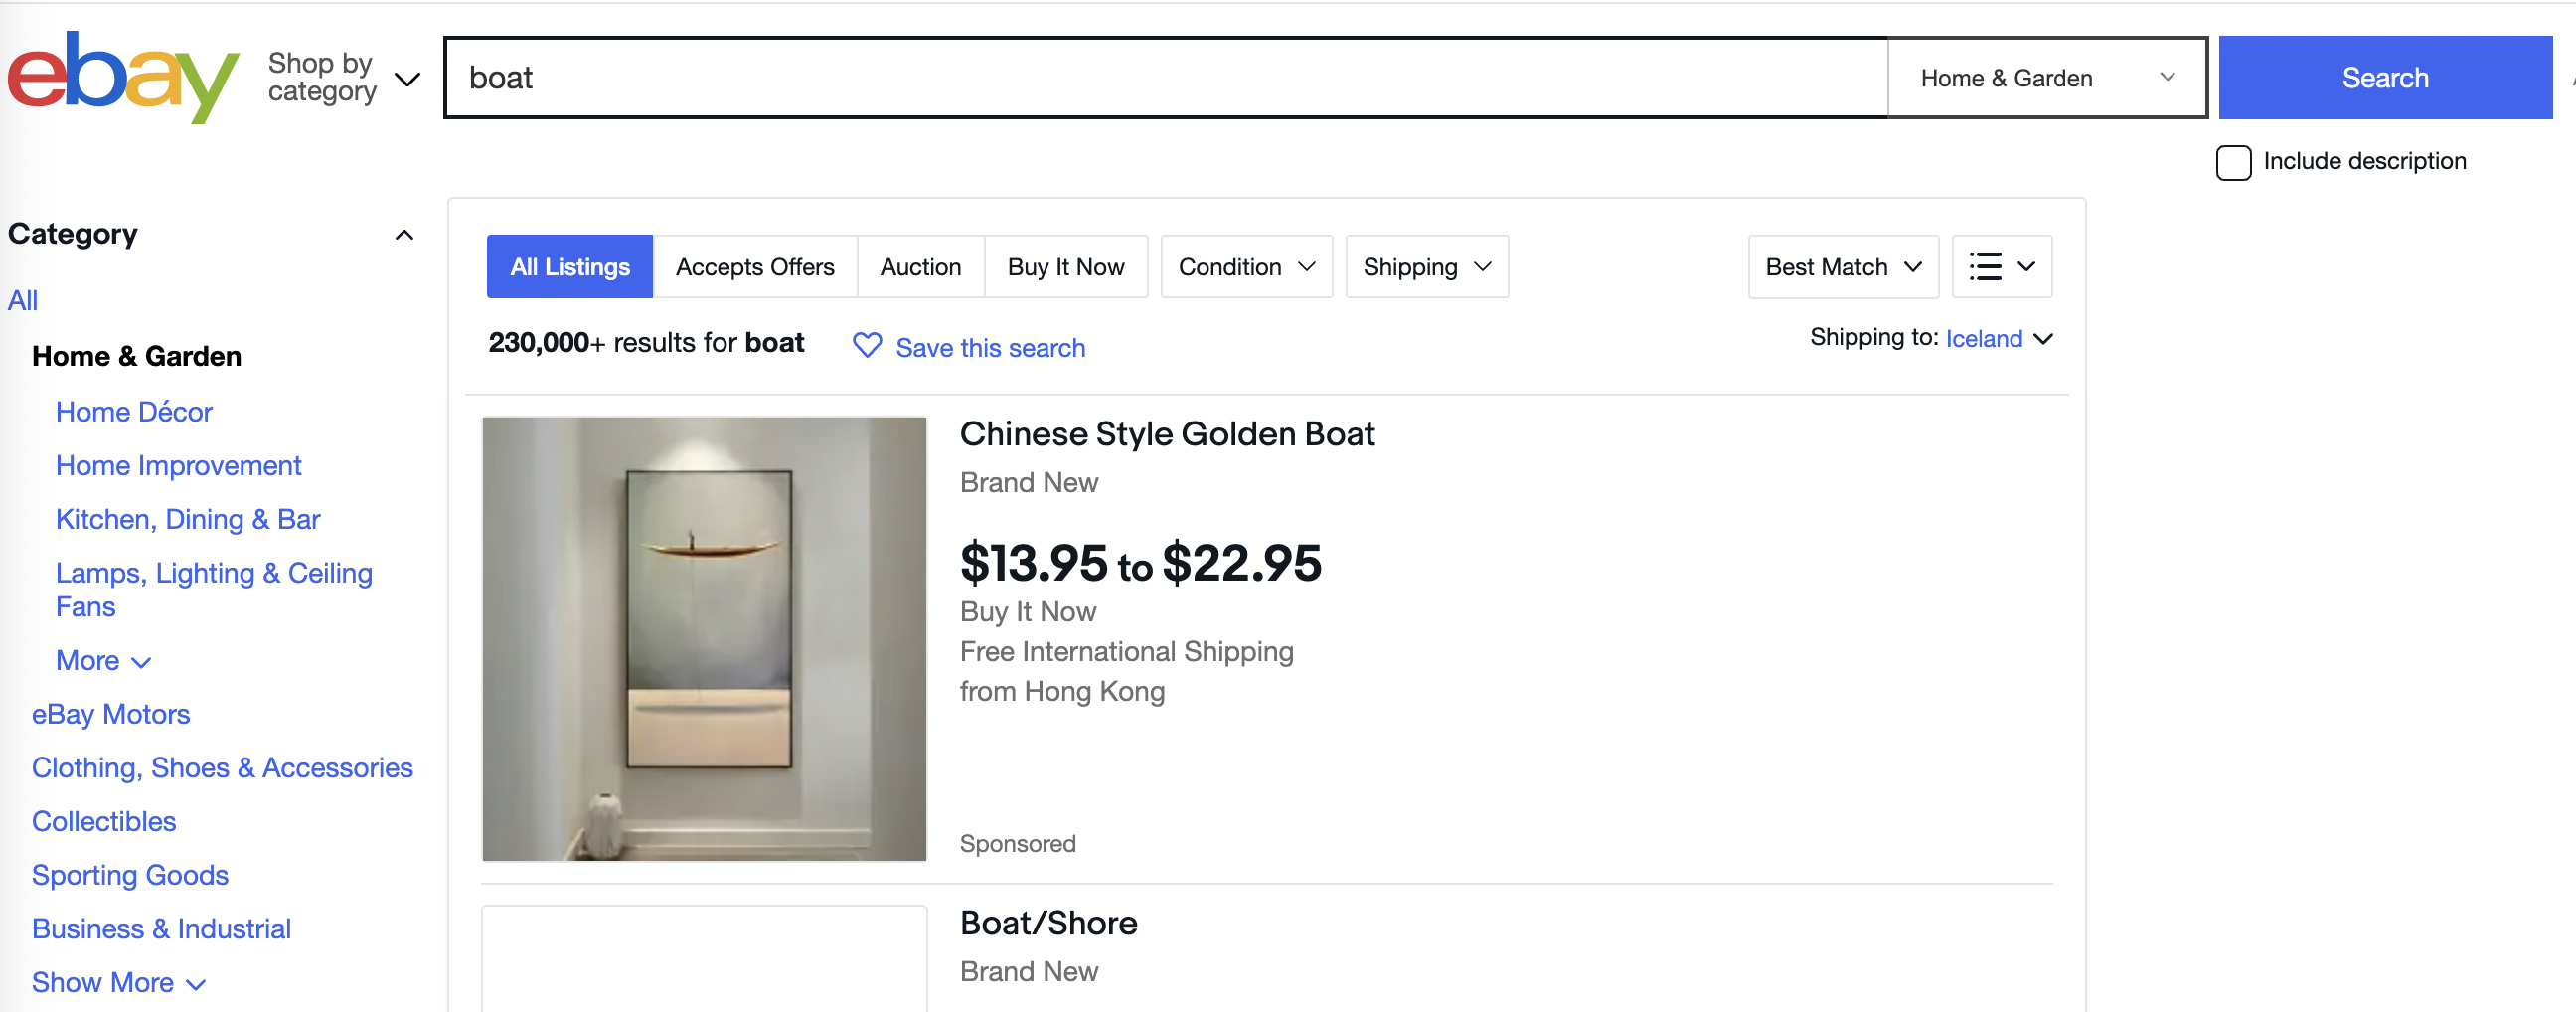
\includegraphics[width=150mm, height=80mm]{Images/benchmarking/search_result_ebay.png}
\captionof{figure}{Ebay's search result page}
    \end{center}
\end{Figure}
One of the metrics we can use is the number of visible search results, Craigslist being the "winner" in that category. Although the number of results might seem important, Bland and Ebay, in our opinion give better results, as they put their focus on the price, which is important to consumers in the used marketplace. Bland in particular uses vibrant colors in their search result for prices, but opt for a black color and less emphasis when viewing the product page. Clearly expecting customers to be drawn into the product based on price from search results. Craigslist focuses on showing you the images of the product, letting that draw you in and never really focusing on the price. Ebays approach is also interesting as they give you only one result in the view but focusing on pricing, availability and the product information. 